\documentclass[../main.tex]{subfiles}

\begin{document}

\subsection{Simulation and reinforcement learning}

% Describe detailed design and implementation of 
% the Proof of Concept (PoC) to prove the feasibility 
% of your design idea and deliver the core of your 
% project solution. It is highly recommended to design 
% and implement the core features of system by choosing 
% the most important/critical use cases (or important 
% component(s) from your high-level design) then design, 
% implement and test them.

% Design and implement part of your complete system. 
% It is expected that the PoC delivers 20% to 30% of 
% the important system use cases.

% Conduct initial PoC tests to demonstrate the 
% feasibility of the design idea of your solution. 
% This will help you refine your design and identify 
% potential technical and logistical issues that you 
% need to address to ensure your project success.

% Demonstrate your PoC to the examiners during the 
% senior project presentation.

\lipsum[1]

\subsection{Object detection}

\lipsum[1]

\subsection{Physical components}

The most critical parts in the hardware
architecture are the Raspberry Pi and the drone. 
So we started by configuring the Raspberry Pi 
\textsc{sd}-card,
flashed it with Ubuntu 18.04 desktop version,
and installed Parrot Olympe successfully. 
Then we plugged in the Wi-Fi dongle adapter
in a \textsc{usb}~2.0 port in the Raspberry Pi, 
and the \textsc{os} discovered it automatically. 

Now everything is ready to test the 
\anafi drone, so we will connect the
Raspberry Pi to the drone using built-in Wi-Fi
to allow Raspberry to send/receive instructions
to the drone. 
For connecting Raspberry Pi and the laptop, 
we used the external Wi-Fi adapter and turned on the hotspot feature to create an access point,
now we can connect to Raspberry Pi and execute 
scripts using \textsc{ssh} protocol.

We executed the takeoff and move forward scripts,
and it worked successfully, so we got the green 
light to continue. 
Regarding the power supply we were thinking of modifying the drone's battery
by removing the plastic shield because of the drone's
payload restrictions and limitations, but everything changed after 
testing the drone's maximum payload. As shown in \cref{fig:payload} below
we attached \SI{190}{\gram} of Raspberry Pi and Arduino boards
to see the effect on the performance and flight and
battery drain percentage. 
The drone has taken off  successfully, 
and the flight was normal but, we faced an expected 
battery drain that went from 
\SI{100}{\percent} to \SI{90}{\percent} in 
\SI{1.5}{\minute}.
This means the drone can fly up to 
\SI{15}{\minute} which is \SI{10}{\minute} 
less than the default battery time 
which will be considered in design constraints.
In our case, the total weight of our parts will be 
less than 
\SI{170}{\gram} 
which will add small time to the battery life.

\begin{figure}[tbp]
	\centering
	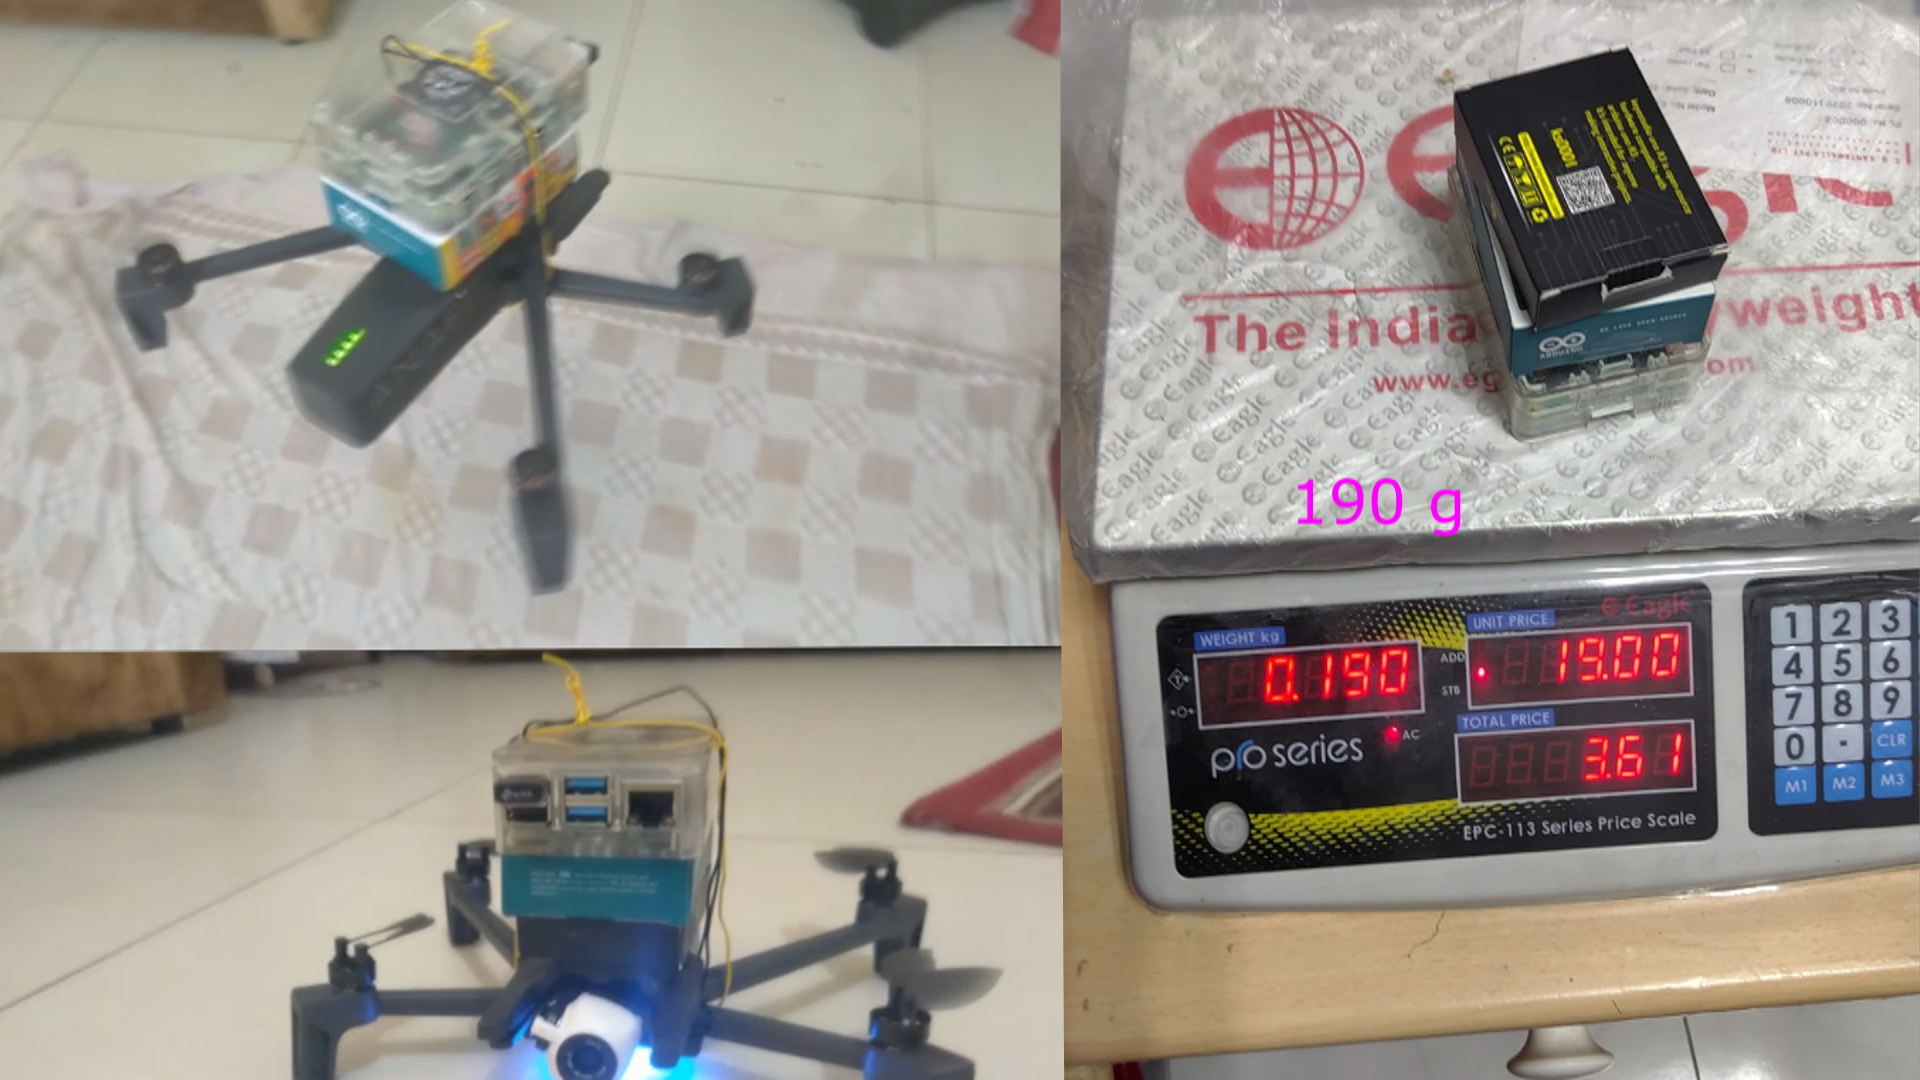
\includegraphics[width=0.6\textwidth]{payload.png}
	\caption{The drone payload}
	\label{fig:payload}
\end{figure} 

For Raspberry Pi power supply it can be connected in 
two different options as shown in \cref{fig:connection}, 
for option A we can use \textsc{usb}-\textsc{A} to power the Raspberry directly without
need to solder any wires,
but there is some internal resistance,
in option B it Power the Raspberry Pi through the \textsc{gpio} 
interface by soldering two wires to the motherboard and 
connect to pin 4 and 6 in the Raspberry Pi board,
this option has small internal resistance compared to option A.
For simplicity, we will choose option A and we will 
follow the instruction of the manufacture by choosing 
the thickest and shortest possible \textsc{usb} cable to reduce 
the cable loss and voltage drops~\cite{makerfocus}. 	 
 
 \begin{figure}[tbp]
 	\centering
 	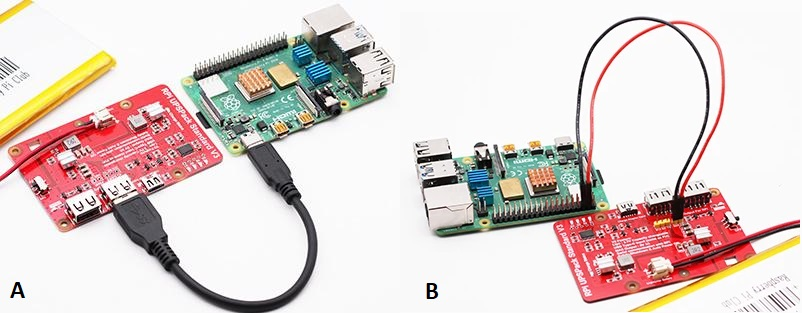
\includegraphics[width=0.6\textwidth]{connection.png}
 	\caption{The Raspberry Pi and power board connection.}
 	\label{fig:connection}
 \end{figure}   

\end{document}
